\documentclass[10pt,twocolumn]{article}
\usepackage[a4paper,margin=18mm,columnsep=6mm]{geometry}
\usepackage{mathptmx}
\usepackage[T1]{fontenc}
\usepackage{amsmath,amssymb}
\usepackage{graphicx}
\usepackage{booktabs}
\usepackage{tabularx}
\usepackage{xcolor}
\usepackage{tikz}
\usetikzlibrary{arrows.meta,positioning,fit,backgrounds,calc}
\usepackage[hidelinks]{hyperref}
\usepackage{cleveref}
\usepackage{caption}
\captionsetup{font=small,labelfont=bf}
\usepackage{enumitem}
\setlist{nosep,leftmargin=*}
\usepackage{listings}
\lstset{basicstyle=\ttfamily\scriptsize,columns=fullflexible,frame=single,framerule=0.3pt,breaklines=true}

%% generated by make_results_tex.py
\newcommand{\todaydate}{October 17, 2026}
\newcommand{\simcoverage}{100\,\%}
\newcommand{\simfree}{64\,m$^2$}
\newcommand{\simdistance}{21.9\,m}
\newcommand{\simgoals}{40}
\newcommand{\simsearchms}{36\,ms}
\newcommand{\resultsabstract}{In an unattended run the robot mapped 47\,m$^2$ of a home in 13\,min, driving 74\,m to 30 frontier goals (1 failed) and drove back to within 0.2\,m of its start without any operator intervention; the frontier search took 50\,ms on the Pi and the whole stack used about 1.5 of the Pi's four cores.}


\title{\textbf{Autonomous Lidar Mapping of a Home with a Low-Cost Tracked Robot:\\
Hector SLAM, Nav2 and Frontier Exploration on a Raspberry~Pi~5}}
\author{Marthens Hakizimana and Amir Taghavipour\\
\small Motion and Power Electronics Control (MPEC) Lab, Simon Fraser University\\
\small BCIT Centre for Welding Technologies and Metallurgy Research}
\date{\small \todaydate}

\begin{document}
\maketitle

\begin{abstract}
\noindent
This paper describes how a low-cost educational tracked robot (Hiwonder MentorPi~T1:
Raspberry~Pi~5, STM32 motor board, Oradar MS200 360\textdegree{} lidar, Deptrum Aurora~930
RGB-D camera) was turned into a robot that maps a house on its own. The robot runs the whole
real-time loop on board: a lidar driver written for this work, Hector SLAM, the ROS~2 Nav2
stack (NavFn planner, Regulated Pure Pursuit controller, layered costmaps, recovery behaviours)
and a frontier explorer that chooses where to go next. A laptop on the same Wi-Fi network only
watches and steers: it shows the camera, the growing map, Nav2's plan, the frontiers and the
goal, and lets the operator pause, take over with the keyboard, send the robot home and save
the map. Obstacle avoidance is layered: the global planner avoids mapped walls, the controller's
local costmap and collision check avoid what the lidar sees now, and the robot's own motor node
refuses to drive into anything closer than 0.25\,m whatever it is told. Bringing the system up
on the real robot exposed problems that no simulation would have shown, the most important being
that the motor signs had been calibrated wrong: the robot drove backwards and turned the wrong way
while its wheel odometry reported the opposite, which corrupted the map within seconds. The
error was found by matching lidar scans before and after a turn and confirmed with the camera.
\resultsabstract
\end{abstract}

\section{Introduction}
Mapping an indoor space is the first step for almost every mobile-robot task: a map is what a
robot localises against, plans in and reports on. With a 2D lidar the mapping itself is a solved
problem \cite{kohlbrecher2011,grisetti2007,hess2016}; what remains costly is the driving. An
operator has to steer the robot slowly through every room, close loops and come back to fill
gaps, and the quality of the map depends on how patiently that is done. Frontier-based
exploration \cite{yamauchi1997} automates this: the robot repeatedly drives to the boundary
between what it has seen and what it has not, until no reachable boundary is left.

This work implements that loop on a low-cost tracked robot and documents the implementation in
enough detail to be repeated. Its contributions are practical rather than algorithmic:
\begin{enumerate}
\item A complete, on-board ROS~2 Jazzy exploration stack for a Raspberry~Pi~5 robot with a
  low-cost lidar: driver, SLAM, Nav2 configuration, a velocity adapter for a controller that takes
  fractions of maximum speed, and a frontier explorer with progress monitoring, blacklisting,
  return-to-home and run logging (\cref{sec:system,sec:explorer}).
\item A distributed split between robot and operator PC, chosen so that a Wi-Fi drop costs
  only the view, never the control loop, with the trade-offs measured (\cref{sec:distributed}).
\item A calibration procedure that uses only the lidar: the robot's true rotation is measured
  by circular cross-correlation of two scans, which revealed inverted motor signs that the
  wheel odometry could not see (\cref{sec:calibration}).
\item An offline simulation of the explorer and a real exploration of a home, with coverage,
  distance, timing and on-board load reported (\cref{sec:results}).
\end{enumerate}

\section{Related work}
\textbf{Lidar SLAM.} Grid-based Rao--Blackwellised particle filters (GMapping
\cite{grisetti2007}) need odometry and many particles; Hector SLAM \cite{kohlbrecher2011}
matches each scan against a multi-resolution occupancy map by Gauss--Newton optimisation and
needs no odometry at all, which suits robots whose wheel odometry is poor, such as tracked
robots that skid when they turn. Cartographer \cite{hess2016} and SLAM Toolbox \cite{macenski2021slam}
add pose-graph loop closure, at a higher computational cost. Hector was chosen here because the
robot's track odometry is unreliable (\cref{sec:calibration}) and because its cost is a few
percent of one Pi core.

\textbf{Navigation.} Nav2 \cite{macenski2020nav2} is the ROS~2 navigation framework: a
behaviour tree sequences a global planner, a local controller and recovery behaviours, all
working on layered costmaps \cite{lu2014layered}. Regulated Pure Pursuit \cite{macenski2023rpp}
follows the global path with a lookahead point and slows down in tight spaces and near
obstacles, which suits slow differential and tracked robots.

\textbf{Exploration.} Yamauchi's frontier exploration \cite{yamauchi1997} drives to the nearest
frontier. Later work weighs information gain against travel cost \cite{gonzalez2002,julia2012}, uses
sampling (RRT-based exploration \cite{umari2017}) or learned policies. ROS packages such as
\texttt{explore\_lite} \cite{horner2016} implement greedy frontier exploration on top of
Nav2. The explorer here is a greedy one with a capped size bonus, written so that every decision
is logged and could be replayed.

\section{Hardware}\label{sec:hardware}
\Cref{tab:hardware} lists the robot. The MentorPi~T1 is a tracked chassis with two JGB37-520
geared motors (1:90, 3960 encoder counts per output turn) driven by an STM32 board (RRC~Lite)
that runs its own speed loop; the firmware used here was built from source and flashed from the
Pi in an earlier lab \cite{lab03}. The lidar sits 0.12\,m above the floor on the robot's centre;
the RGB-D camera looks forward 0.07\,m ahead of it.

\begin{table}[t]
\centering\small
\caption{robot04 and the operator PC.}\label{tab:hardware}
\begin{tabularx}{\columnwidth}{@{}lX@{}}
\toprule
Computer & Raspberry Pi 5, 8\,GB, Ubuntu 24.04, ROS~2 Jazzy \\
Motor board & Hiwonder RRC Lite (STM32), own firmware, encoder speed loop \\
Drive & 2 tracks, JGB37-520 1:90; top speed used 0.153\,m/s (50\,\% of motor maximum) \\
Lidar & Oradar MS200: 360\textdegree, 10\,Hz, 0.03--12\,m, USB serial 230\,400 baud \\
Camera & Deptrum Aurora 930: RGB 640$\times$400 + aligned depth, 15\,fps \\
Battery & 2S Li-ion, 7.0--8.4\,V \\
Operator PC & Laptop, Ubuntu 22.04, ROS~2 Humble, same Wi-Fi network \\
Middleware & Cyclone DDS on both machines, domain 17 \\
\bottomrule
\end{tabularx}
\end{table}

\section{System architecture}\label{sec:system}
\Cref{fig:architecture} shows the nodes and where they run. Everything that closes a control
loop runs on the robot; the PC runs only the operator interface.

\begin{figure*}[t]
\centering
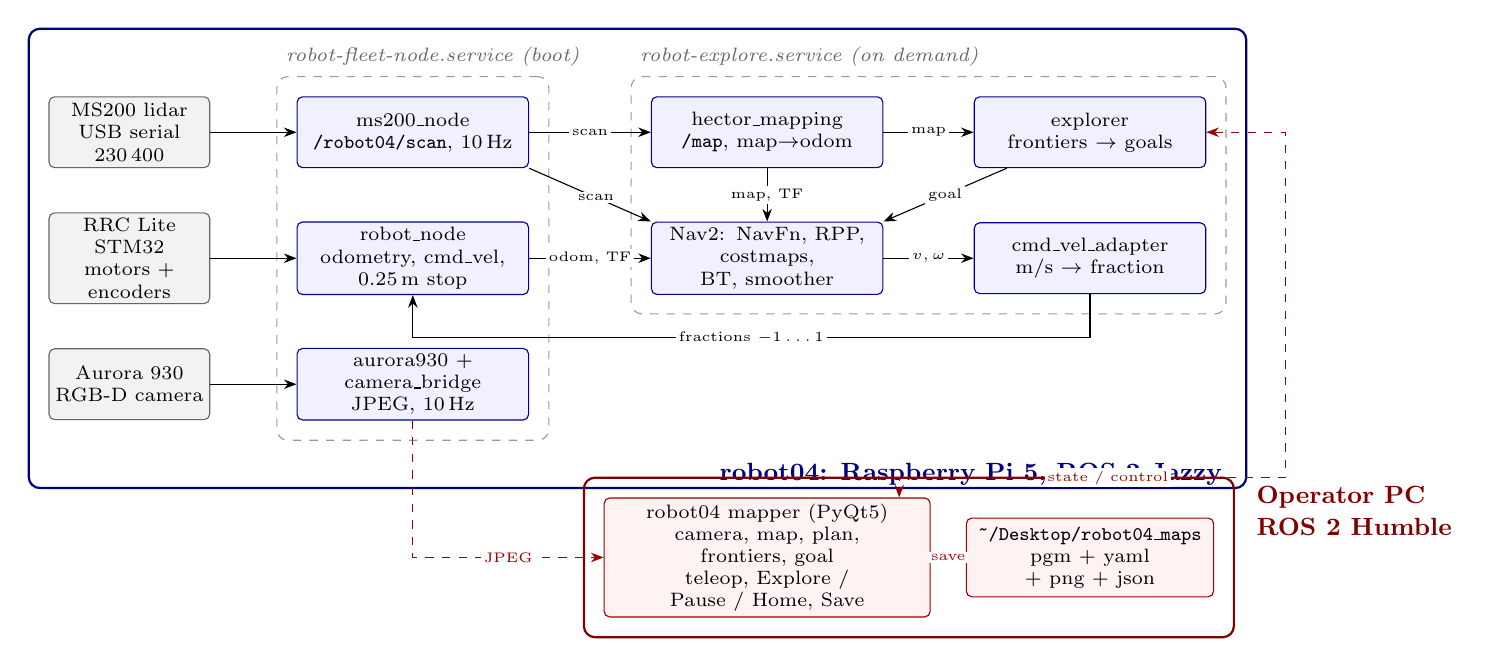
\begin{tikzpicture}[x=1cm,y=1cm,
  box/.style={draw=blue!60!black,rounded corners=2pt,fill=blue!6,align=center,font=\scriptsize,minimum height=9mm,text width=28mm,inner sep=2pt},
  hw/.style={draw=black!60,rounded corners=2pt,fill=black!5,align=center,font=\scriptsize,minimum height=9mm,text width=19mm,inner sep=2pt},
  pc/.style={draw=red!60!black,rounded corners=2pt,fill=red!5,align=center,font=\scriptsize,minimum height=10mm,text width=40mm,inner sep=2pt},
  ar/.style={-{Stealth[length=1.6mm]},thin},
  wifi/.style={-{Stealth[length=1.6mm]},thin,red!60!black,dashed},
  lab/.style={font=\tiny,fill=white,inner sep=1pt},
  grp/.style={font=\scriptsize\itshape,text=black!60,anchor=south west}]
% hardware
\node[hw] (lidar) at (0,0) {MS200 lidar\\USB serial 230\,400};
\node[hw] (board) at (0,-1.6) {RRC Lite STM32\\motors + encoders};
\node[hw] (cam)   at (0,-3.2) {Aurora 930\\RGB-D camera};
% boot service
\node[box] (ms200)  at (3.6,0)    {ms200\_node\\\texttt{/robot04/scan}, 10\,Hz};
\node[box] (robot)  at (3.6,-1.6) {robot\_node\\odometry, cmd\_vel, 0.25\,m stop};
\node[box] (bridge) at (3.6,-3.2) {aurora930 + camera\_bridge\\JPEG, 10\,Hz};
% explore service
\node[box] (hector)   at (8.1,0)    {hector\_mapping\\\texttt{/map}, map$\to$odom};
\node[box] (nav2)     at (8.1,-1.6) {Nav2: NavFn, RPP,\\costmaps, BT, smoother};
\node[box] (explorer) at (12.2,0)   {explorer\\frontiers $\to$ goals};
\node[box] (adapter)  at (12.2,-1.6){cmd\_vel\_adapter\\m/s $\to$ fraction};
% group frames
\node[draw=black!40,dashed,rounded corners,fit=(ms200)(bridge),inner sep=2.5mm] (g1) {};
\node[grp] at (g1.north west) {robot-fleet-node.service (boot)};
\node[draw=black!40,dashed,rounded corners,fit=(hector)(adapter),inner sep=2.5mm] (g2) {};
\node[grp] at (g2.north west) {robot-explore.service (on demand)};
\node[draw=blue!50!black,thick,rounded corners,fit=(lidar)(cam)(g1)(g2),inner xsep=2.5mm,inner ysep=6mm] (pi) {};
\node[font=\small\bfseries,text=blue!50!black,anchor=north east] at ($(pi.south east)+(-0.2,0.45)$) {robot04: Raspberry Pi 5, ROS 2 Jazzy};
% PC
\node[pc] (app)  at (8.1,-5.4) {robot04 mapper (PyQt5)\\camera, map, plan, frontiers, goal\\teleop, Explore / Pause / Home, Save};
\node[pc,text width=30mm] (maps) at (12.2,-5.4) {\texttt{\textasciitilde/Desktop/robot04\_maps}\\pgm + yaml + png + json};
\node[draw=red!50!black,thick,rounded corners,fit=(app)(maps),inner xsep=2.5mm,inner ysep=2.5mm] (pcbox) {};
\node[font=\small\bfseries,text=red!50!black,anchor=north west] at ($(pcbox.north east)+(0.15,0)$) {Operator PC};
\node[font=\small\bfseries,text=red!50!black,anchor=north west] at ($(pcbox.north east)+(0.15,-0.4)$) {ROS 2 Humble};
% robot-side arrows
\draw[ar] (lidar) -- (ms200);
\draw[ar] (board) -- (robot);
\draw[ar] (cam) -- (bridge);
\draw[ar] (ms200) -- node[lab]{scan} (hector);
\draw[ar] (ms200.south east) -- node[lab,pos=.55]{scan} (nav2.north west);
\draw[ar] (hector) -- node[lab]{map} (explorer);
\draw[ar] (hector) -- node[lab]{map, TF} (nav2);
\draw[ar] (explorer) -- node[lab]{goal} (nav2.north east);
\draw[ar] (nav2) -- node[lab]{$v,\omega$} (adapter);
\draw[ar] (adapter.south) -- ++(0,-0.55) -| node[lab,pos=.25]{fractions $-1\ldots1$} (robot.south);
\draw[ar] (robot) -- node[lab]{odom, TF} (nav2);
% Wi-Fi arrows
\draw[wifi] (bridge.south) |- node[lab,pos=.75]{JPEG} (app.west);
\draw[wifi,{Stealth[length=1.6mm]}-{Stealth[length=1.6mm]}] (explorer.east) -- ++(1.0,0) |- node[lab,pos=.75]{state / control} ($(app.north east)+(0,0.25)$) -- ($(app.north east)+(-0.4,0.25)$) -- ($(app.north east)+(-0.4,0)$);
\draw[wifi] (app.east) -- node[lab]{save} (maps.west);
\end{tikzpicture}
\caption{Nodes and their placement. Solid arrows stay on the robot; dashed arrows cross Wi-Fi.
The robot's boot service runs the drivers; the exploration service is started from the PC when
needed. The operator PC never sits inside a control loop.}
\label{fig:architecture}
\end{figure*}

\subsection{Drivers (boot service)}
\textbf{ms200\_node.} The MS200 streams 47-byte packets (header \texttt{0x54 0x2C}, rotation
speed, start angle, 12 points of range and intensity, end angle, time stamp, CRC-8 with polynomial
0x4D) at 230\,400 baud. No ROS~2 Jazzy driver was available, so one was written: a reader thread
checks the CRC, interpolates the angle of each of the 12 points between the start and end angle,
detects the end of a revolution when the angle wraps, and bins each revolution into 450 fixed
rays (0.8\textdegree), keeping the nearest return per ray. Device angles are clockwise and are
negated, so the published \texttt{LaserScan} is counter-clockwise from the robot's front as ROS
expects. Returns closer than 0.10\,m are dropped: the robot's own frame appears at 0.03--0.09\,m.
A udev rule matching both the USB IDs and the USB port gives the lidar a stable name
(\texttt{/dev/lidar}), because the robot's voice module uses the same CH340 serial chip.

\textbf{robot\_node.} Takes \texttt{cmd\_vel} with \texttt{linear.x} and \texttt{angular.z} as
fractions $-1\ldots1$ of the configured maximum speed (not m/s), mixes them per track
(left $= f - t$, right $= f + t$), and publishes encoder odometry and the TF
\texttt{robot04/odom}$\to$\texttt{robot04/base\_footprint} at 20\,Hz. It stops 0.5\,s after the
last command, and before and while driving it checks the lidar sector $\pm25^\circ$ around the
direction of travel: closer than 0.25\,m it refuses to move. That check is independent of
everything above it and is the last layer of obstacle avoidance.

\textbf{Camera.} The vendor driver publishes RGB and depth; \texttt{camera\_bridge} turns them
into a 480-pixel JPEG stream (10\,Hz, only while someone subscribes). The driver occasionally
stops delivering frames, so the bridge restarts it after 6\,s without a frame.

\subsection{SLAM}
\texttt{hector\_mapping} (the ROS~2 port by RobotX Workshops) builds a 1024$\times$1024 grid at
5\,cm (51\,m square) with two resolution levels and publishes \texttt{map}$\to$\texttt{robot04/odom},
so that the encoder odometry remains the child transform and Nav2 can use both. It is configured
with a range window of 0.12--8\,m and updates the map every 0.2\,m or 0.06\,rad.

\subsection{Navigation}
Nav2's controller, planner, behaviour, velocity-smoother and BT-navigator servers are started
directly (not through \texttt{nav2\_bringup}) with one parameter file. The main choices:
\begin{itemize}
\item \textbf{Footprint}: a circle of radius 0.15\,m (body $\approx0.24\times0.20$\,m).
\item \textbf{Global costmap} (map frame): Hector's map as static layer, the live scan as obstacle
  layer, inflation 0.45\,m, unknown space tracked. \textbf{NavFn} plans with A* and
  \texttt{allow\_unknown}, because frontier goals sit at the edge of the unknown.
\item \textbf{Local costmap} (odom frame, rolling 3$\times$3\,m, 10\,Hz): live scan only, inflation
  0.40\,m. Its update rate must not be lower than the controller rate (\cref{sec:lessons}).
\item \textbf{Controller}: Regulated Pure Pursuit at 8\,Hz, 0.10\,m/s, lookahead 0.25--0.6\,m,
  rotate-to-heading at 0.6\,rad/s when the path turns more than 0.6\,rad, linear speed
  regulated by curvature and by costmap cost, and a collision check that stops the robot if the
  path up to the carrot would collide within 1.5\,s.
\item \textbf{Goal checker}: 0.20\,m, any heading (the lidar sees all round).
\item \textbf{Transform tolerance} 1.0\,s, because Hector stamps \texttt{map}$\to$\texttt{odom}
  with the time of the scan it was computed from, 0.1--0.2\,s in the past.
\end{itemize}

\subsection{Velocity adapter}
Nav2 commands $v$ (m/s) and $\omega$ (rad/s); robot\_node expects fractions. With the measured
top speed $v_{\max}=0.153$\,m/s and effective track width $b=0.105$\,m (\cref{sec:calibration}),
\begin{equation}
f = \frac{v}{v_{\max}},\qquad t = \frac{\omega\, b}{2\,v_{\max}},\qquad
\ell = f - t,\quad r = f + t .
\end{equation}
The motor speed loop does not move a track below about 0.1 of its maximum, so each non-zero
track fraction is raised to at least 0.12 (with its sign), and both are scaled down together if
one exceeds 1, which keeps the curvature. The adapter is muted until the explorer starts and
whenever the operator pauses, so manual teleop and Nav2 never command the motors at the same time.

\section{Frontier explorer}\label{sec:explorer}
The explorer is a 400-line Python node. Once per second it reads the robot pose from TF
(\texttt{map}$\to$\texttt{base\_footprint}) and every 3\,s it searches the latest map.

\textbf{Frontier search.} Cells are free ($0\le p\le25$), occupied ($p\ge65$) or unknown ($-1$).
The search works on the known part of the map only (a margin of 20 cells around it), because
the 1024$\times$1024 grid is mostly unknown. Steps:
\begin{enumerate}
\item Clearance: Euclidean distance transform of the non-occupied cells, in metres.
\item Traversable cells: free cells with clearance $\ge$ the robot radius (0.15\,m).
\item Reachability: 8-connected Dijkstra from the traversable cell nearest the robot gives the
  geodesic distance $d$ to every reachable cell.
\item Frontier cells: free cells with an unknown 4-neighbour, grouped into 8-connected clusters;
  clusters shorter than 0.30\,m are ignored.
\item Goal of a cluster: among reachable cells within 0.35\,m of the cluster, the one nearest its
  centroid. Clusters with no such cell are unreachable and skipped.
\item Score $= d_{\text{goal}} - 0.5\min(L, 1.5\,\text{m})$, with $L$ the cluster length. The
  lowest score wins: the nearest frontier, with a bonus for larger openings. The bonus is
  capped because the ragged edge of a long scan can merge into one cluster tens of metres long,
  whose bonus would otherwise dominate (observed in the first run: a 38.9\,m ``frontier'').
\end{enumerate}

\textbf{Goal handling.} The winner becomes a \texttt{NavigateToPose} goal facing away from the
robot. While it is active, each new search checks whether a frontier still exists within 0.6\,m
of the goal's frontier centroid; if not, the area has been seen on the way and the goal is
cancelled in favour of the next one (``explored''). A goal fails when Nav2 aborts it, when the
robot has not moved 0.15\,m or turned 0.5\,rad for 30\,s, or after a timeout of
$40\,\text{s} + 2.5\,d/0.05\,\text{m/s}$. Failed goals and their frontiers are blacklisted
(0.4\,m radius). Goals that are \emph{reached} are blacklisted too: a frontier that is still
there when the robot stands next to it is a pocket the lidar cannot see into, typically under
furniture, and without this rule the robot re-sent the same goal 39 times in two minutes.

\textbf{Termination and safety.} When three searches in a row find no reachable frontier, the
robot drives back to its start and the map is saved (map\_server format). The run also ends at a
time limit (45\,min) and the robot returns home when the battery falls below 7.0\,V. Every event
(goal sent, reached, explored, failed, with timing, distance and pose) and a sample every 5\,s
(explored area, frontier count, battery) are written to a JSON-lines log; the results in
\cref{sec:results} are computed from it.

\textbf{Operator control.} The PC sends \texttt{start}, \texttt{pause}, \texttt{stop},
\texttt{home} and \texttt{save} on \texttt{/robot04/explore/control}. Any teleop key, the STOP
button or the space bar sends \texttt{pause} first, which cancels the Nav2 goal and mutes the
velocity adapter, so the operator always wins.

\begin{figure}[t]
\centering
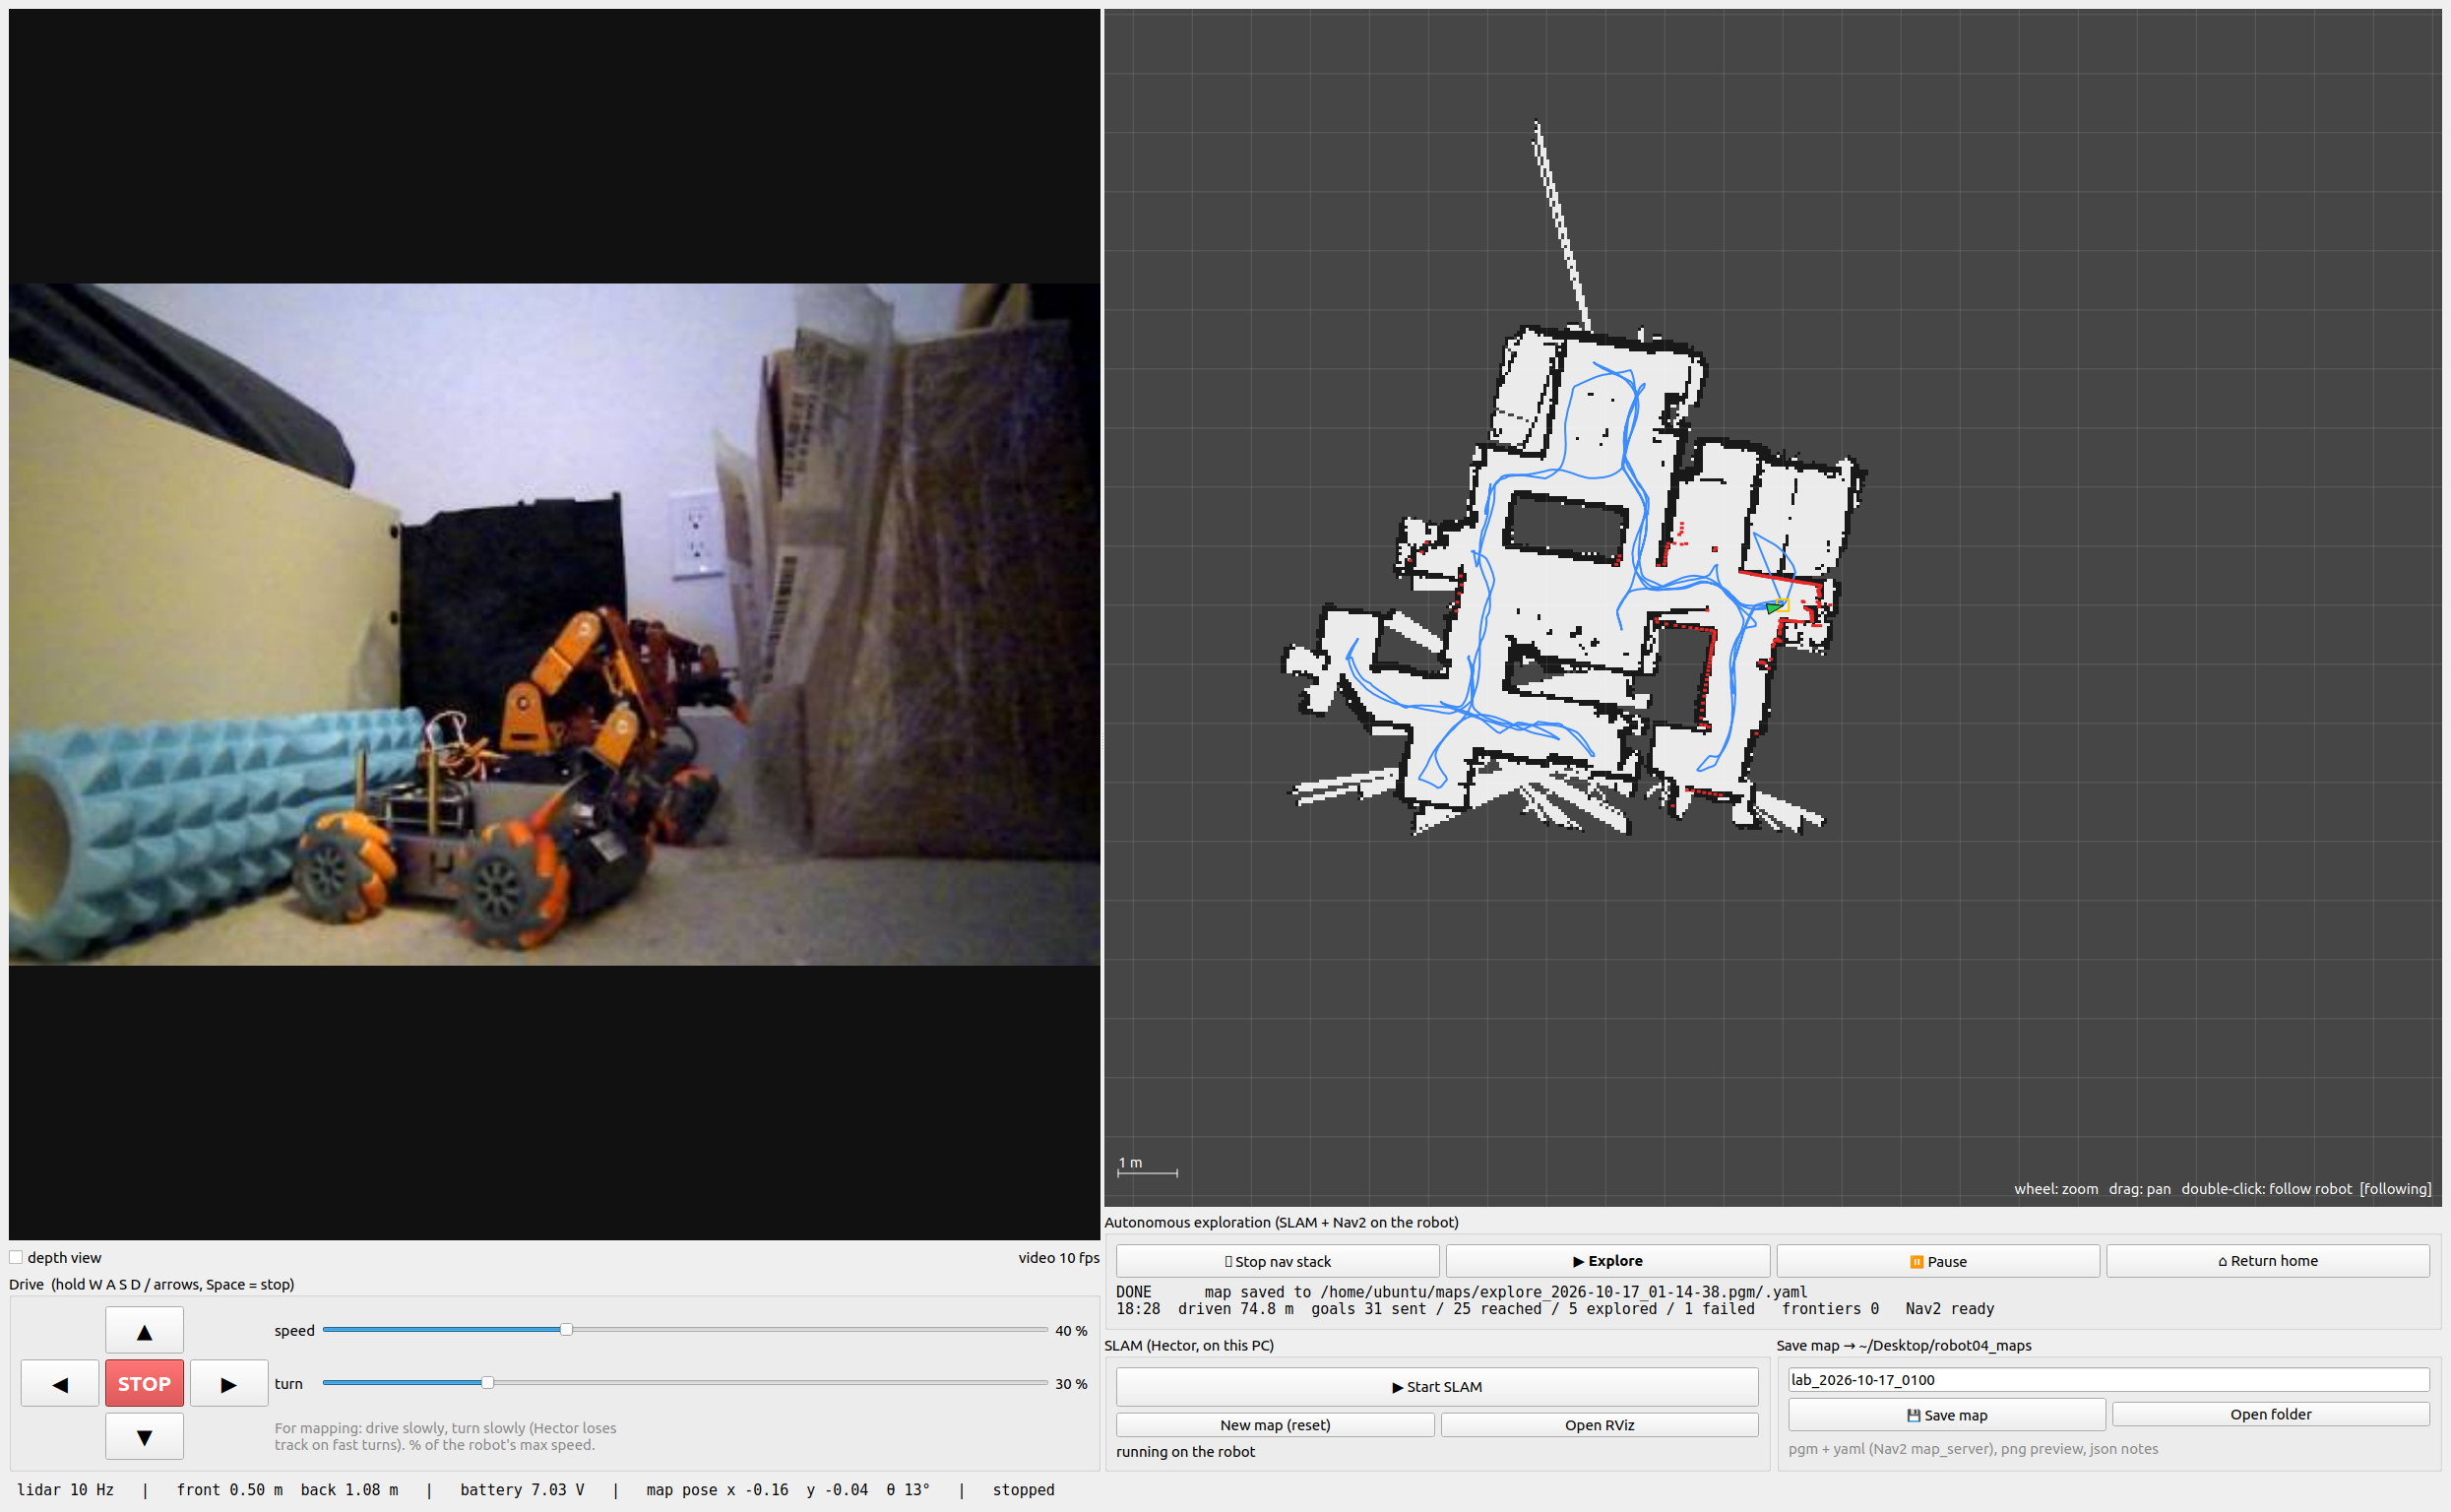
\includegraphics[width=\columnwidth]{figures/mapper_app.png}
\caption{The operator application at the end of the run: camera and teleop (left); live map with the robot's
SLAM path, Nav2 plan, goal, frontiers and start (right); exploration, SLAM and saving controls (bottom).}
\label{fig:app}
\end{figure}

\section{Distributing the work}\label{sec:distributed}
Two placements were considered: everything except the drivers on the PC (the robot as a
sensor head), or everything that closes a loop on the robot (the PC as a viewer). The first
mapping sessions ran Hector on the PC and worked: a scan is about 2\,KB, 20\,KB/s over Wi-Fi,
and the measured extra latency was about 6\,ms. For autonomous driving the second placement was
chosen because a Wi-Fi drop of more than 0.5\,s would otherwise stop the robot (robot\_node's
command timeout) or, worse, leave the controller acting on stale localisation; with everything on
board a drop costs only the view. The cost is CPU on the Pi, measured in \cref{tab:cpu}: the
whole stack uses about 1.5 of the Pi's 4 cores, at 52\,\textdegree C without throttling.
The camera driver and the explorer's Python search are the largest single loads; the explorer
(and with it the global planner) is the natural candidate to move to the PC if the Pi ever
becomes the bottleneck, because neither is time-critical. It was not moved because Humble's and
Jazzy's \texttt{NavigateToPose} action types differ (Jazzy adds error fields to the result), so a
Humble client and a Jazzy server do not interoperate reliably.

\begin{table}[t]
\centering\small
\caption{CPU use on the Pi 5 while exploring (percent of one core, \texttt{top}, 2\,s average).}\label{tab:cpu}
\begin{tabular}{@{}lr@{}}
\toprule
Process & CPU \% \\
\midrule
aurora930 camera driver & 26 \\
explorer (Python, frontier search) & 21 \\
robot\_node (Python, odometry + safety) & 17 \\
camera\_bridge (JPEG) & 9 \\
bt\_navigator & 9 \\
planner\_server (NavFn + global costmap) & 7 \\
controller\_server (RPP + local costmap) & 6 \\
ms200\_node & 5 \\
behavior\_server, velocity\_smoother, lifecycle & 11 \\
hector\_mapping & 3 \\
cmd\_vel\_adapter & 3 \\
\midrule
Total (of 400) & $\approx$ 150 \\
\bottomrule
\end{tabular}
\end{table}

\textbf{Middleware.} The PC used Cyclone DDS and the robot's services Fast DDS. That worked for
the sensor topics, but two problems disappeared only when the robot's services were switched to
Cyclone as well: the camera bridge stopped receiving frames after the camera driver had been
restarted (a new process subscribing to the same topic received them; Fast DDS shared-memory
transport is the likely cause, and UDP-only transport also fixed it), and the explorer's state
messages arrived at the PC garbled. Deserialisation warnings that remain between Humble and
Jazzy come from \texttt{/parameter\_events}, whose type differs between the two distributions,
and are harmless.

\section{Calibration: what the wheels did not say}\label{sec:calibration}
The first autonomous runs produced maps with walls drawn twice at different angles. A rotation
test showed why: commanded to turn left at 0.2 of full speed for 20\,s, the robot's encoder
odometry reported $+383^\circ$ and Hector reported $-678^\circ$. Either the lidar was mirrored or
the robot turned the other way from what its odometry believed.

To decide without trusting either, the rotation was measured from the lidar alone. With scans
$A$ (before) and $B$ (after a short turn) as range vectors over the 450 rays, the rotation is
the circular shift $k^\ast$ that best aligns them,
\begin{equation}
k^\ast = \arg\min_k \operatorname{median}_{i}\bigl|A_i - B_{i+k}\bigr| ,\qquad
\Delta\psi = k^\ast \cdot 0.8^\circ ,
\end{equation}
over rays valid in both. Because the lidar's angle convention had been checked against the
camera (objects to the left of the image appear at positive angles), this measurement is
trustworthy. It said the robot turned \emph{right} when told to turn left, which a
before/after camera frame confirmed (the scene moved left in the image). A second test, the
change of the range straight ahead after driving ``forward'', showed that the robot also drove
backwards. Both motor signs had been inverted when the robot was first set up; because the
odometry uses the same signs, it reported the commanded motion, not the real one, and nothing
looked wrong until a sensor that does not share the motors' sign convention was compared.

\begin{table}[t]
\centering\small
\caption{Rotation measured by scan alignment vs.\ encoder odometry, 1.5\,s turns.}\label{tab:calib}
\begin{tabular}{@{}lrrr@{}}
\toprule
Command & Scan & Encoders & Note \\
\midrule
\multicolumn{4}{@{}l}{\emph{before the fix} ($+1/-1$, $b=0.17$\,m)} \\
turn $+0.25$ & $-51.2^\circ$ & $+28.5^\circ$ & wrong way \\
turn $-0.25$ & $+44.8^\circ$ & $-28.8^\circ$ & wrong way \\
\multicolumn{4}{@{}l}{\emph{after the fix} ($-1/+1$, $b=0.10$\,m)} \\
turn $+0.25$ & $+43.2^\circ$ & $+46.8^\circ$ & \\
turn $-0.25$ & $-47.2^\circ$ & $-50.3^\circ$ & \\
turn $+0.40$ & $+81.6^\circ$ & $+85.3^\circ$ & \\
turn $-0.40$ & $-86.4^\circ$ & $-88.5^\circ$ & \\
\bottomrule
\end{tabular}
\end{table}

\Cref{tab:calib} shows the measurements. After flipping both signs, the scan-measured rotation
averaged 0.954 of the encoder estimate with track width 0.10\,m, so the effective track width on
carpet is $0.105$\,m, well below the 0.17\,m between the track centres: a tracked robot turning in
place skids, and the effective width absorbs that. The linear speed was measured with the
encoders at 0.3 and 0.6 of full speed (0.047 and 0.091\,m/s, i.e.\ $0.153\,f$\,m/s) and checked
against the lidar range to a wall; below about 0.1 of full speed the tracks do not move.

\section{Results}\label{sec:results}
\subsection{Simulation}
The explorer's frontier logic was first run offline (\texttt{tools/sim\_explore.py}): a
synthetic 10$\times$7\,m apartment with five rooms, a ray-cast 360\textdegree{} lidar with 450
rays and 8\,m range, an occupancy grid written from the rays, and a robot that follows the
geodesic path to the chosen goal and re-plans every 0.5\,m. There is no SLAM error and no
controller, so this tests the choice of goals and termination only. The robot mapped
\simcoverage\ of the \simfree\ of free space after \simdistance\ of driving and \simgoals\
frontier goals; a frontier search took \simsearchms\ on the laptop (\cref{fig:sim}). Coverage
rises quickly while the robot crosses open rooms and then flattens as it visits the last corners,
the usual shape for greedy exploration.

\begin{figure}[t]
\centering
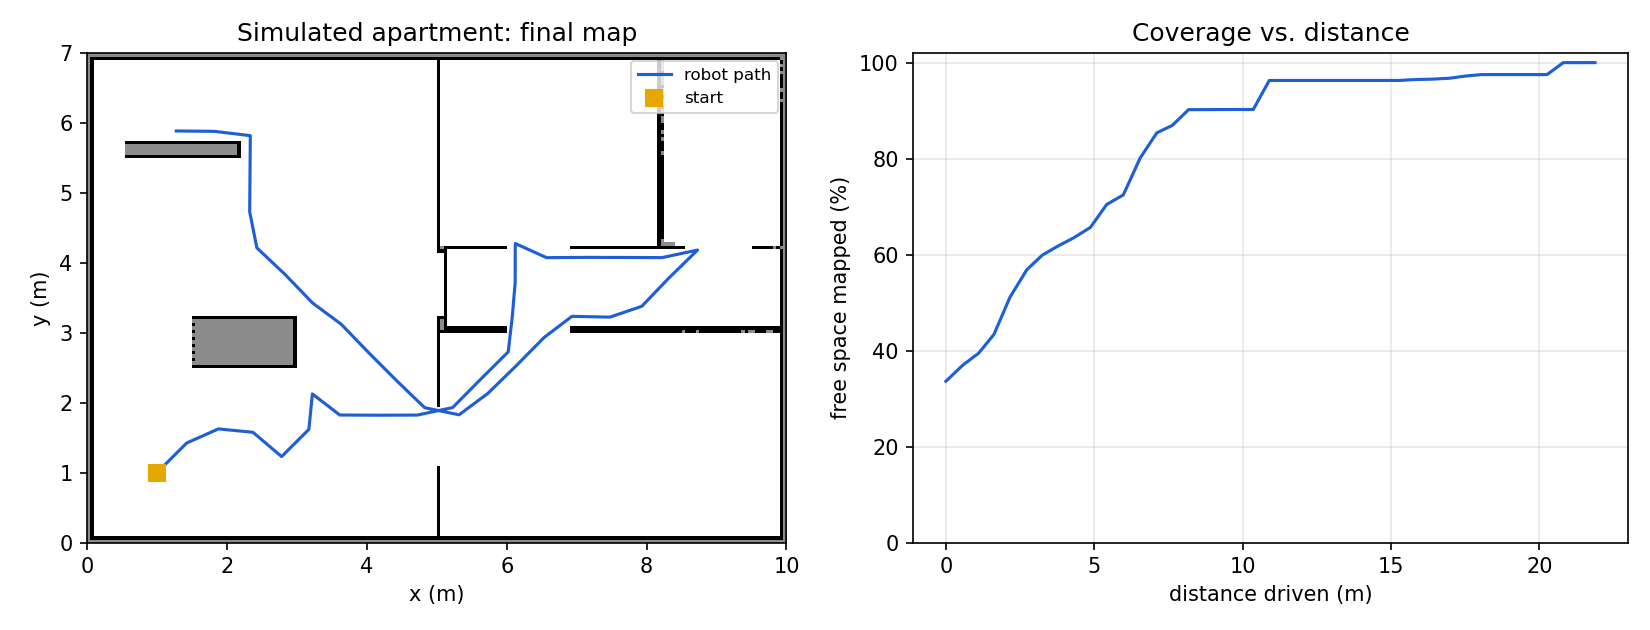
\includegraphics[width=\columnwidth]{figures/sim_explore.png}
\caption{Offline simulation: final map and path (left), free space mapped against distance driven (right).}
\label{fig:sim}
\end{figure}

%% generated by make_results_tex.py
\subsection{Autonomous run in a home}
The robot was placed in a carpeted hallway of a furnished apartment at night with the room lights on, the exploration service was started from the PC and Explore was pressed once; nobody touched the robot or the keyboard afterwards. Doors stood as they were left; there are no stairs on this floor. \Cref{tab:run} summarises the run, \cref{fig:runmap} shows the saved map with the path the robot chose and \cref{fig:progress} the mapped area over time. Of the 30 goals sent, 24 were reached and 5 were cancelled because the frontier behind them was seen on the way; 1 failed (timeout after 156 s). Mapped area grows fastest in the first two minutes, when every goal opens a new room to the 360\textdegree{} lidar, and creeps up afterwards as the robot visits the corners and gaps behind furniture one at a time; the number of open frontiers peaks at about four and a half minutes and falls to zero after 11.6 minutes, when the robot returned to its start. The single failure was a goal on the far side of a wall that the planner could reach only through unknown space; the controller made progress but not enough, and the goal was dropped after its timeout of 156\,s. The mean speed over the run, 0.098\,m/s, is close to the controller's cruise speed of 0.10\,m/s, so the time was spent driving rather than waiting or recovering. The long white streak at the top of the map is free space seen along a few rays through a narrow gap (most likely a door left ajar); the frontier at its end is a ray or two wide, below the 0.30\,m minimum frontier length, so the explorer ignored it, which is also why the room behind it is missing from the map.

\begin{table}[t]
\centering\small
\caption{The autonomous run, from the explorer's log.}\label{tab:run}
\begin{tabular}{@{}lr@{}}
\toprule
Duration (start to end) & 12.6 min \\
Mapped area (known cells) & 47.3 m$^2$ \\
Free / occupied area in the saved map & 37.5 / 9.8 m$^2$ \\
Map extent & 10.9 $\times$ 13.2 m \\
Path length (SLAM poses, 5\,cm steps) & 74.0 m \\
Mean speed over the run & 0.098 m/s \\
Frontier goals sent & 30 \\
\quad reached & 24 \\
\quad seen on the way (cancelled) & 5 \\
\quad failed (blacklisted) & 1 \\
Operator interventions & 0 \\
Frontier search on the Pi, mean / max & 50 / 58 ms \\
Candidate frontiers per search, mean & 11.1 \\
Mapping rate & 3.8 m$^2$/min \\
Battery, start / end & 7.40 / 7.08 V \\
How it ended & back at the start \\
\bottomrule
\end{tabular}
\end{table}

\begin{figure}[t]
\centering
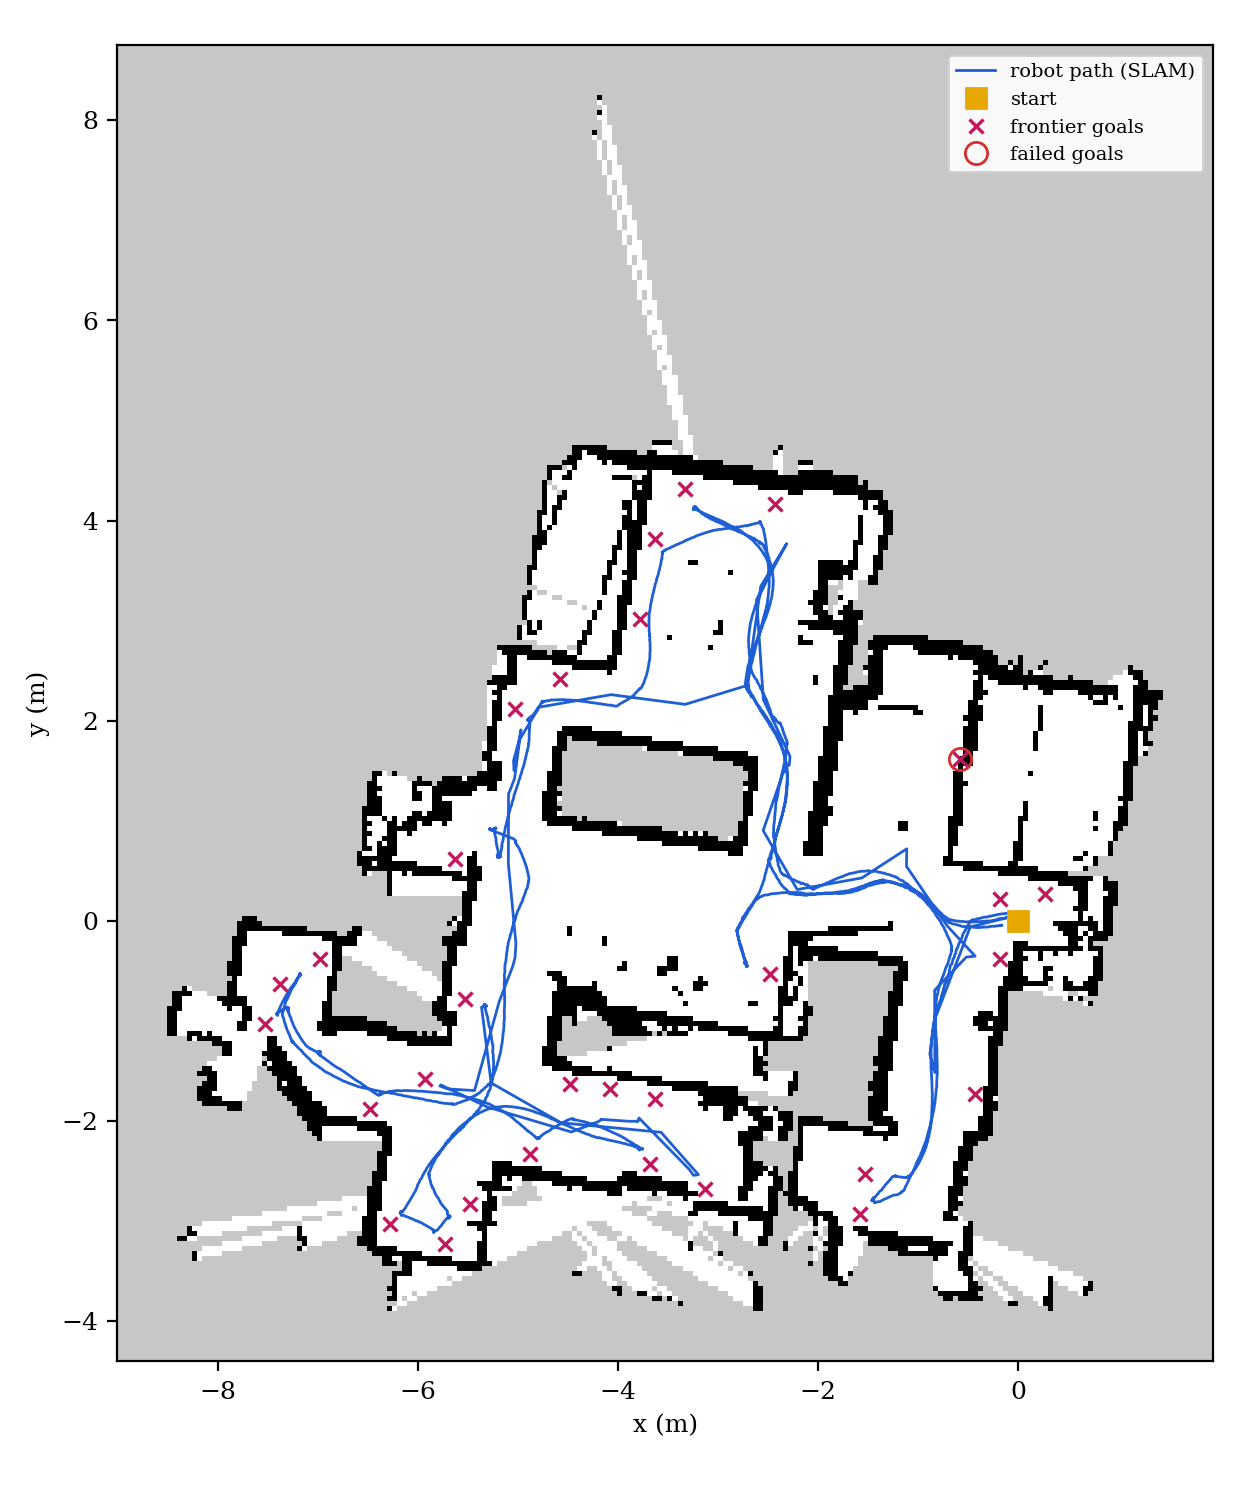
\includegraphics[width=\columnwidth]{figures/run_map.png}
\caption{Map saved at the end of the autonomous run (5\,cm cells; white free, black occupied, grey unknown), with the robot's path from SLAM, its start and the frontier goals it chose.}\label{fig:runmap}
\end{figure}

\begin{figure}[t]
\centering
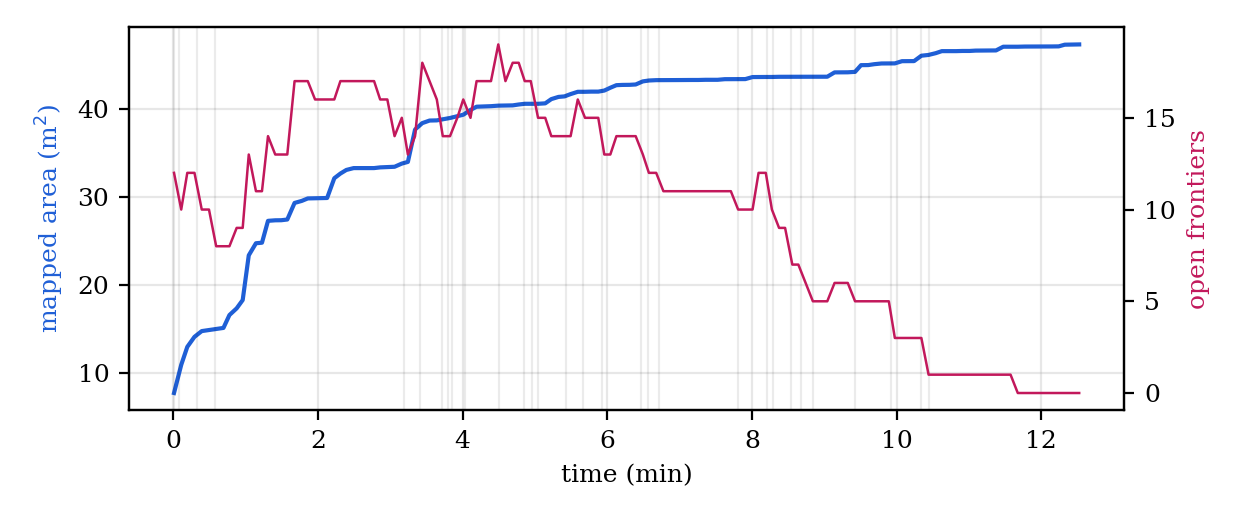
\includegraphics[width=\columnwidth]{figures/run_progress.png}
\caption{Mapped area (blue) and open frontiers (red) during the run; grey lines mark goals sent.}\label{fig:progress}
\end{figure}


\section{Lessons from bringing it up}\label{sec:lessons}
The algorithms worked as published; the time went into the interfaces between them.
\begin{itemize}
\item \textbf{Check motion against a sensor that does not share its conventions.} Wheel
  odometry computed with the same signs as the motor commands will always agree with the
  commands. Two minutes of scan alignment found what weeks of teleop had not.
\item \textbf{A controller cannot run faster than its costmap.} With the local costmap at 5\,Hz
  and the controller at 10\,Hz, Nav2's controller waited for the costmap and ran at 5--6\,Hz,
  which looked like an overloaded CPU. The Pi was at 40\,\%.
\item \textbf{SLAM time stamps lag.} Hector's \texttt{map}$\to$\texttt{odom} carries the scan
  time; with Nav2's default transform tolerance the controller intermittently could not
  transform the robot pose and aborted goals.
\item \textbf{Namespaces.} An action client created in namespace \texttt{/robot04} with the
  relative name \texttt{navigate\_to\_pose} looks for \texttt{/robot04/navigate\_to\_pose}; the
  explorer waited for a server that was there all along under the root namespace.
\item \textbf{Frontiers that cannot be cleared.} Reaching a frontier does not always remove it;
  without blacklisting reached goals the explorer looped.
\item \textbf{Mixed DDS implementations} are supported in principle and fragile in practice;
  using the same one on every machine removed two unrelated faults at once.
\end{itemize}

\section{Reproducing the run}\label{sec:reproduce}
All code is in the repository given below. On the robot, after the drivers' boot service is running:
\begin{lstlisting}
sudo apt install ros-jazzy-navigation2 ros-jazzy-nav2-bringup \
     ros-jazzy-laser-geometry python3-scipy
cd ~/ros2_ws/src && git clone \
  https://github.com/RobotX-Workshops/hector_slam_ros2.git
# copy ros2/mentorpi_nav from the repository here, then
cd ~/ros2_ws && colcon build --packages-up-to \
  hector_mapping mentorpi_nav --cmake-args -DCMAKE_BUILD_TYPE=Release
cp src/mentorpi_nav/systemd/robot-explore.service \
   ~/.config/systemd/user/
systemctl --user daemon-reload; sudo loginctl enable-linger ubuntu
\end{lstlisting}
On the PC, \texttt{pc/robot04-mapper/run.sh} opens the application of \cref{fig:app}; \emph{Start nav stack on
robot} and \emph{Explore} start a run. Afterwards the log (\texttt{\textasciitilde/explore\_logs}) and the saved
map (\texttt{\textasciitilde/maps}) are turned into the figures and tables of \cref{sec:results} by
\texttt{tools/analyze\_run.py} and \texttt{make\_results\_tex.py}; \texttt{tools/sim\_explore.py} reproduces
\cref{fig:sim}.

\section{Limitations and future work}
The 2D lidar sees a horizontal plane 12\,cm above the floor: it cannot see a drop-off (stairs),
low obstacles such as cables or flat toys, or overhangs such as table tops above the robot's
height but below its camera. In this house there were no stairs on the mapped floor; elsewhere
a no-go zone or a depth-camera cliff check is needed before the robot is left alone. Hector
has no loop closure, so a long loop through several rooms can leave a visible seam; SLAM
Toolbox would add it at a higher CPU cost. The explorer is greedy and does not trade
information gain against travel; a next step is to weigh frontiers by the unknown area expected
behind them and to use the depth camera for 3D obstacles.

\section{Conclusion}
A low-cost tracked robot with a Raspberry~Pi~5 and an entry-level 360\textdegree{} lidar can map a home on its own with
standard ROS~2 components, provided the parts are configured for each other: a lidar driver,
Hector SLAM, Nav2 with Regulated Pure Pursuit and layered costmaps, a velocity adapter for a
motor controller that speaks in fractions, and a frontier explorer that blacklists what it cannot
clear. Running every loop on the robot and using the PC only to watch and steer means a Wi-Fi
drop costs the operator's view rather than the robot's control loop (by design; dropouts
were not provoked in this study), at a cost of about 1.5 of the Pi's four cores. The most
consequential fault was not in any algorithm but in the robot's motor signs, and it was found by
the simplest test: compare what the wheels say with what the lidar sees.

\paragraph{Code.} \url{https://github.com/hmarthens1/rpi5-robot-board}: \texttt{ros2/mentorpi\_robot}
(drivers), \texttt{ros2/mentorpi\_nav} (explorer, adapter, Nav2 configuration, simulation),
\texttt{pc/robot04-mapper} (operator application).

\begin{thebibliography}{99}\small
\bibitem{kohlbrecher2011} S.~Kohlbrecher, O.~von Stryk, J.~Meyer, U.~Klingauf, ``A flexible and scalable SLAM system with full 3D motion estimation,'' \emph{IEEE Int.\ Symp.\ Safety, Security and Rescue Robotics (SSRR)}, 2011.
\bibitem{grisetti2007} G.~Grisetti, C.~Stachniss, W.~Burgard, ``Improved techniques for grid mapping with Rao-Blackwellized particle filters,'' \emph{IEEE Trans.\ Robotics}, 23(1), 2007.
\bibitem{hess2016} W.~Hess, D.~Kohler, H.~Rapp, D.~Andor, ``Real-time loop closure in 2D LIDAR SLAM,'' \emph{IEEE ICRA}, 2016.
\bibitem{macenski2021slam} S.~Macenski, I.~Jambrecic, ``SLAM Toolbox: SLAM for the dynamic world,'' \emph{Journal of Open Source Software}, 6(61), 2021.
\bibitem{macenski2020nav2} S.~Macenski, F.~Mart\'in, R.~White, J.~Gin\'es Clavero, ``The Marathon 2: A navigation system,'' \emph{IEEE/RSJ IROS}, 2020.
\bibitem{lu2014layered} D.~V.~Lu, D.~Hershberger, W.~D.~Smart, ``Layered costmaps for context-sensitive navigation,'' \emph{IEEE/RSJ IROS}, 2014.
\bibitem{macenski2023rpp} S.~Macenski, S.~Singh, F.~Mart\'in, J.~Gin\'es, ``Regulated pure pursuit for robot path tracking,'' \emph{Autonomous Robots}, 47, 2023.
\bibitem{yamauchi1997} B.~Yamauchi, ``A frontier-based approach for autonomous exploration,'' \emph{IEEE CIRA}, 1997.
\bibitem{gonzalez2002} H.~H.~Gonz\'alez-Ba\~nos, J.-C.~Latombe, ``Navigation strategies for exploring indoor environments,'' \emph{Int.\ J.\ Robotics Research}, 21(10--11), 2002.
\bibitem{julia2012} M.~Juli\'a, A.~Gil, O.~Reinoso, ``A comparison of path planning strategies for autonomous exploration and mapping of unknown environments,'' \emph{Autonomous Robots}, 33, 2012.
\bibitem{umari2017} H.~Umari, S.~Mukhopadhyay, ``Autonomous robotic exploration based on multiple rapidly-exploring randomized trees,'' \emph{IEEE/RSJ IROS}, 2017.
\bibitem{horner2016} J.~H\"orner, ``Map-merging for multi-robot system,'' Bachelor's thesis, Charles University, Prague, 2016 (\texttt{explore\_lite}).
\bibitem{lab03} M.~Hakizimana, ``Lab 03: encoder motors and speed control,'' \texttt{rpi5-ros2-rrclite} lab notes, 2026.
\end{thebibliography}

\end{document}
